%!TeX root=../tese.tex
%("dica" para o editor de texto: este arquivo é parte de um documento maior)
% para saber mais: https://tex.stackexchange.com/q/78101

\chapter{Resultados}
\label{chap:resultados}

É apresentada nessa seção uma comparação entre as previsões realizadas pelos modelos
testados neste trabalho. Foram realizados experimentos com diferentes 
combinações de parâmetros, detalhadas no capítulo \ref{chap:experimentos},
nesta seção é utilizado o modelo que apresentou melhor desempenho de cada uma 
das classes de algoritmos testadas: regressão linear, redes \textit{multilayer feed forward},
redes recorrentes e redes bidirecionais.

É possível comparar o desempenho dos modelos a partir da tabela \ref{tab:compara_modelos}.

\begin{table}[H]
    \centering
    \begin{tabular}{llll}
        \toprule
        Modelo & MAE     & RMSE    & MAPE \\
        \midrule
        Regressão linear & 26435 & 38970 & 0.32  \\
        Rede \textit{multilayer feed forward} & 25520.8 & 42929.2 & 0.25  \\
        Rede recorrente & 22694 & 43918 & 0.19  \\
        Rede bidirecional & 19185 & 33942 & 0.17 \\
        \bottomrule
    \end{tabular}
    \caption{Desempenho dos modelos de regressão linear}
    \label{tab:compara_modelos}
\end{table}

Na análise da tabela acima, nota-se que o desempenho nas previsões
melhora à medida que se aumenta a robustez do modelo.

Observa-se uma significativa melhora de 13\% da regressão linear para os modelos
de redes recorrentes, reflexo da capacidade de reconhecer sequências e contexto.
A melhora também se reflete nos erros absolutos calculados pela MAE, contudo a 
RMSE apresentou piora em relação à regressão linear, provavelmente por conta 
de \textit{outliers}, uma vez que a RMSE é mais sensível a valores discrepantes.

As redes bidirecionais apresentaram melhor desempenho em comparação com os outros 
modelos, em virtude da arquitetura mais complexa com duas redes recorrentes. Há 
redução de 2\% da MAPE em relação às redes recorrentes e de 15\% em relação à 
regressão linear. Esse comportamento se reflete, também, nos indicadores de 
erro absoluto que são os menores entre as classes de algoritmos testados.

Será utilizado o estado de São Paulo para comparar as previsões realizadas 
pelo modelo e o valor real do consumo, a escolha se deu por 
se tratar do maior consumidor de cimento no Brasil. A evolução do consumo 
mensal de cimento em São Paulo pode ser vista na figura \ref{consumo-sp}.

\begin{figure}[H]
    \centering
    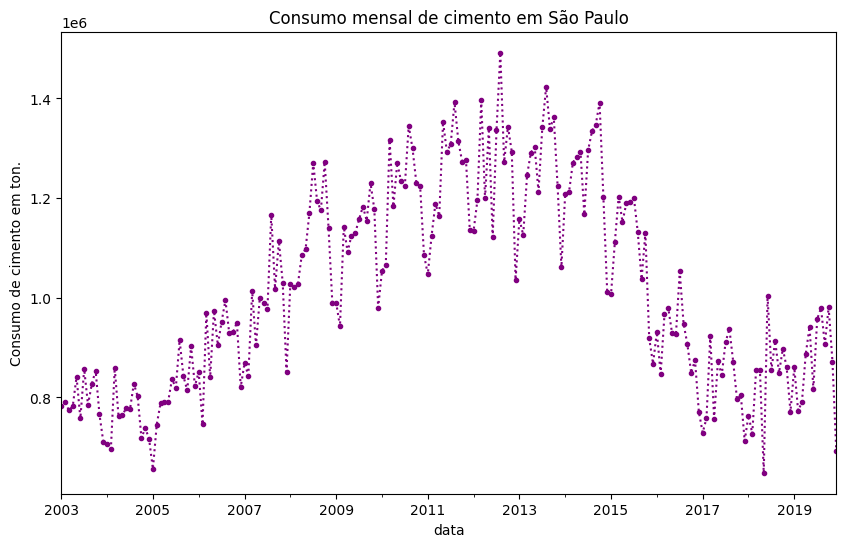
\includegraphics[width=10cm]{../figuras/graficos/evolucao-consumo-sp.png}
    \caption{Evolução do consumo mensal de cimento em São Paulo}
    \label{consumo-sp}
\end{figure}

Na imagem acima, os círculos representam as medições mensais do consumo de 
cimento em São Paulo, observa-se que a demanda por cimento no estado vinha em tendência
de queda desde 2013 e passou a apresentar alta de 2018 em diante.


\section{Regressão linear}

